\documentclass{../UTNetLab}

\title{Bridges, LANs and the Cisco IOS}
\authorshort{A. Khonsari, A. HajiAliKhamseh'i, M. Borhani, A. Khordadi, S. Kashipazha}
\author{%
    Dr. Ahmad Khonsari\\
    \FR{دکتر احمد خونساری}\\
    \mail{a\_khonsari@ut.ac.ir}
    \end{tabular}\vskip 1em
    \begin{tabular}[t]{c}
    Amir Haji Ali Khamseh'i\\
    \FR{امیر حاجی‌علی‌خمسه‌ء}\\
    \mail{khamse@ut.ac.ir}
    \and
    {Muhammad Borhani}\\
    \FR{محمد برهانی}\\
    \mail{m.borhani@ut.ac.ir}
    \and
    {AmirAhmad Khordadi}\\
    \FR{امیراحمد خردادی}\\
    \mail{a.a.khordadi@ut.ac.ir}
    \and
    {Sina Kashipazha}\\
    \FR{سینا کاشی‌پزها}\\
    \mail{sina\_kashipazha@ut.ac.ir}
    \and
    {Hadi Safari}\\
    \FR{هادی صفری}\\
    \mail{hadi.safari@ut.ac.ir}
    \and
    % {alii}\\
    % \FR{دیگران}\\
    % \mail{info@example.com}
}

\begin{document}
\section*{Exercises on Cisco IOS}
    Each group in the lab uses two workstations, a bridge, and two hubs, which are required to be connected as shown in Fig. 3.7, Table 3.2 and Table 3.3.

\section{Network setup}
    In this exercise we build the connection to the router.

    Identify the cable from your workstation and the cable from your router interface (see Fig. 3.7, Table 3.2 and Table 3.3).
    Plug these two cables into your hub.
    In this case, you have built a LAN segment with a \textit{star} topology.
    Your partner should build a star LAN segment on the other side of the router.

    \begin{table}[H]
        \caption{Router and Host IP addresses for Fig. 3.7}
        \centering
        \begin{tabular}{ *2c|*2c|*2c }
            \hline \hline
            \multicolumn{2}{c|}{Router} & \multicolumn{2}{c|}{Host\textsubscript{A}} & \multicolumn{2}{c}{Host\textsubscript{B}} \\
            eth0 & eth1 & Name & IP Address & Name & IP Address \\
            \hline 
            128.238.61.1/24 & 128.238.61.2/24 & h0 & 128.238.61.100/24 & h1 & 128.238.61.101/24 \\
            % 128.238.62.2/24 & 128.238.62.3/24 & h2 & 128.238.62.102/24 & h3 & 128.238.62.103/24 \\
            % 128.238.63.3/24 & 128.238.63.4/24 & h4 & 128.238.63.104/24 & h5 & 128.238.63.105/24 \\
            % 128.238.64.4/24 & 128.238.64.5/24 & h6 & 128.238.64.106/24 & h7 & 128.238.64.107/24 \\
            \hline \hline
            \end{tabular}
    \end{table}

    \begin{figure}[H]
        \centering
        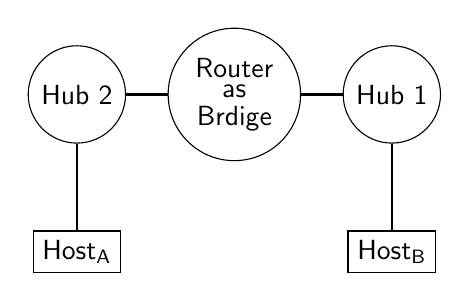
\begin{tikzpicture}[font=\sf]
            \node[draw] (h1) at (-2,-2){Host\textsubscript{A}};
            \node[draw,circle] (hub2) at (-2,0){Hub 2};
            \node[draw,circle] (router) at (0,0){\shortstack{Router\\as\\Brdige}};
            \node[draw,circle] (hub1) at (2,0){Hub 1};
            \node[draw] (h0) at (2,-2){Host\textsubscript{B}};
        
            \draw[thick] (h0) -- (hub1);
            \draw[thick] (h1) -- (hub2);
            \draw[thick] (hub1) -- (router);
            \draw[thick] (hub2) -- (router);
        \end{tikzpicture}
        \caption{\textit{Figure 3.7.} Using a transparent bridge.}        
    \end{figure}

\section{IOS Console}
    Open Router Console (Use telnet to router in physical devices).
    You should now be in the \textit{User EXEC} mode.

    Type \lstinline[language={cisco}]{help} to learn how to use the online help.
    Study Fig. 3.6. Navigate through the \textit{User EXEC}, \textit{Privileged EXEC}, \textit{Global Configuration}, and \textit{Interface Configuration} modes. In each mode, type \lstinline[language={cisco}]{?} to display a list of available commands and study these commands.

    Type \lstinline[language={cisco}]{show version} in the \textit{User EXEC} mode to display the Cisco IOS banner.
    Identify which Cisco IOS Release is running in the router.
    Save the Cisco IOS banner for your lab report.
    
    \subsection*{Report}
    Submit the Cisco IOS banner you saved.
    Identify the release of the Cisco IOS software in the router.

\section*{A simple bridge experiment}
    Figure 3.7 shows a simple case of the use of bridges, which consists of two network segments connected by a bridge.
    With this simple topology, we can easily capture initial BPDUs before each bridge is engaged in the spanning tree calculation.

    Configure transparent bridging as in Fig.
    3.7, Table 3.2 and Table 3.3.
    Note that the default configuration of the hosts and the bridges are different from those in the tables.
    You need to change the IP addresses of the bridge interfaces,\footnote{As soon as you change the IP address of the bridge interface your host is connected to, the \lstinline{telnet} connection will be lost.
    You need to again change the IP address of your workstation to be in the same subnet as the bridge interface. See Section 3.3.3.} as well as set the bridge group and enable the spanning tree algorithm (see the previous section on bridge configuration).
    Do the following experiments.

\section{Bridge packet}
    Configure the IP addresses of your workstation and the bridge interfaces as shown in Fig. 3.7, Table 3.2 and Table 3.3.
    To avoid confusion, each bridge should be configured by only one person.

    Config Cisco Router as transparent Bridge:
    \begin{lstlisting}[language={cisco}]
config term
no ip routing
bridge 1 protocol ieee # for STP protocol
int f0/0
ip addr 128.238.61.1 255.255.255.0
bridge-group 1
no shut
int f0/1
ip addr 128.238.61.2 255.255.255.0
bridge-group 1
no shut
Ctrl+Z
    \end{lstlisting}
    
    Run \lstinline{tcpdump -en ip proto 1} on your machine, and your partner’s machine. Send \lstinline{ping} messages to your partner’s machine: \lstinline[emph={your-host, remote-host}]{ping -sv remote-machine}.
    After receiving the tenth echo reply, quit the \lstinline{ping} process, and save the \lstinline{tcpdump} outputs from both machines.

    During this exercise, don’t run \lstinline{ping} programs at the same time. For clean results, do your experiments in turn.
    
    \subsection*{Report}
    What are the IP and MAC addresses of a packet that went from your machine to the bridge?
    What are the IP and MAC addresses of a packet that went from the router to your partner’s machine?

    Answer the same questions, but for the echo reply that was returned from your partner’s machine.

    Using the \lstinline{tcpdump} outputs from both machines, calculate the average delay that a packet experienced in the bridge.
    Note that the system times of the two machines might be different.
    Show all the steps and submit the \lstinline{tcpdump} outputs with your report.


\section{STP/BPDU packet}
    Run \lstinline{tcpdump -e -c 5 ether multicast} on your workstation to capture 5 BPDUs messages generated by the bridge.
    Save the BPDUs for the lab report.

    You need to collect all the different BPDUs from all group in your lab.
    At this time, save your BPDU capture output. 
    In our next step,  you get BPDUs from other gropu.

    You should collect four different BPDUs in this exercise for all group.
    These BPDUs will be helpful when studying the spanning tree algorithm later in this chapter.

    \subsection*{Report}
    How frequently (in seconds) does a bridge sends its BPDUs?

    Submit the four different BPDUs you saved.
    Identify the values of root ID, root path cost, bridge ID, and port ID for each BPDU\footnote{You may check the physical addresses of network interfaces. You need the MAC addresses to help analyze the BPDUs.} (may need to check BPDU message format Fig.3.4).

    \begin{figure}[H]
        \centering
        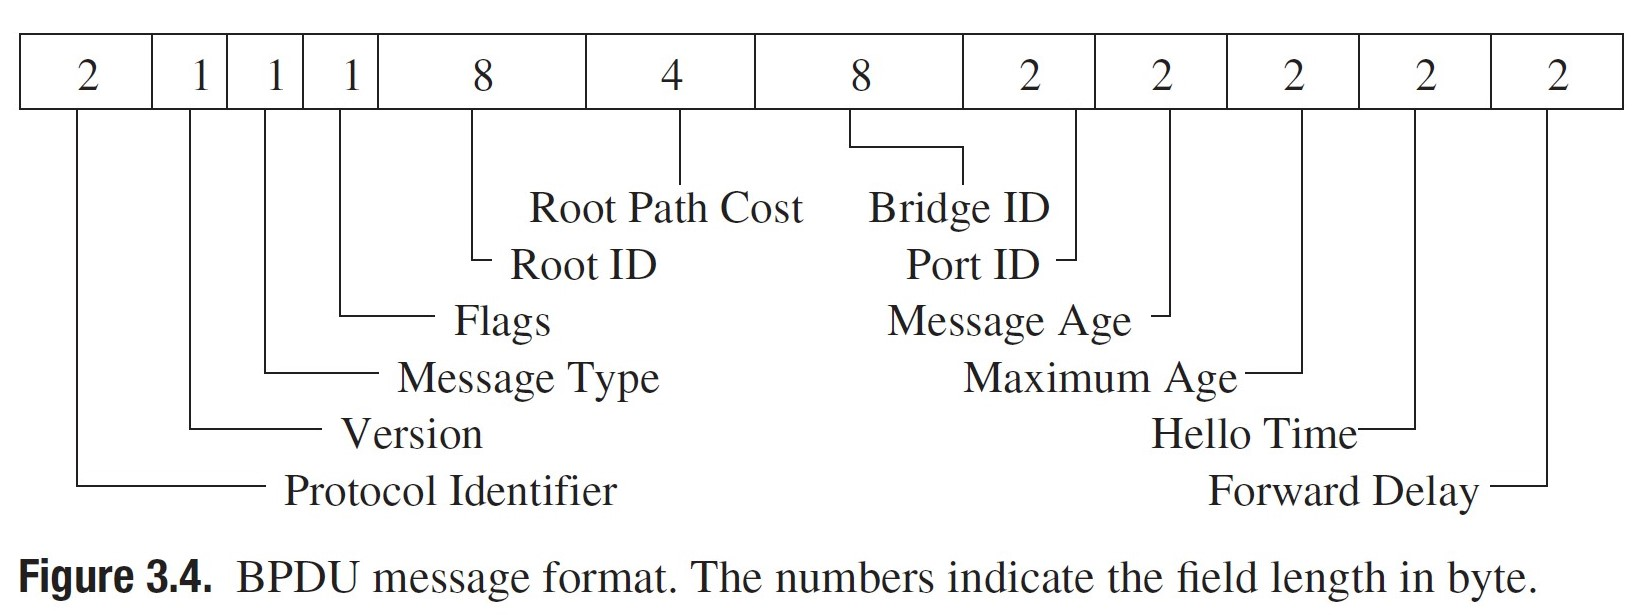
\includegraphics[width=0.9\textwidth]{img/figure3-4.jpg}
        \caption{\textit{Figure 3.4.} BPDU message format. The numbers indicate the field length in byte.}
    \end{figure}

\section*{Spanning tree exercises}
\label{sec:spanning-tree}
    In this section, we will use Fig. 3.8 as our network topology.
    You need to change the IP addresses of the bridge interfaces, as well as that of your workstation. Refer to Section      on how to configure a transparent bridge.
    Also see Section 3.3.3 on how to handle a frozen telnet session after you change the bridge IP address.

    Upon being started, a transparent bridge learns the network topology by analyzing source addresses of incoming frames from all attached networks.
    The next exercise shows the process by which a transparent bridge builds its filtering database.
    \begin{figure}[H]
        \centering
        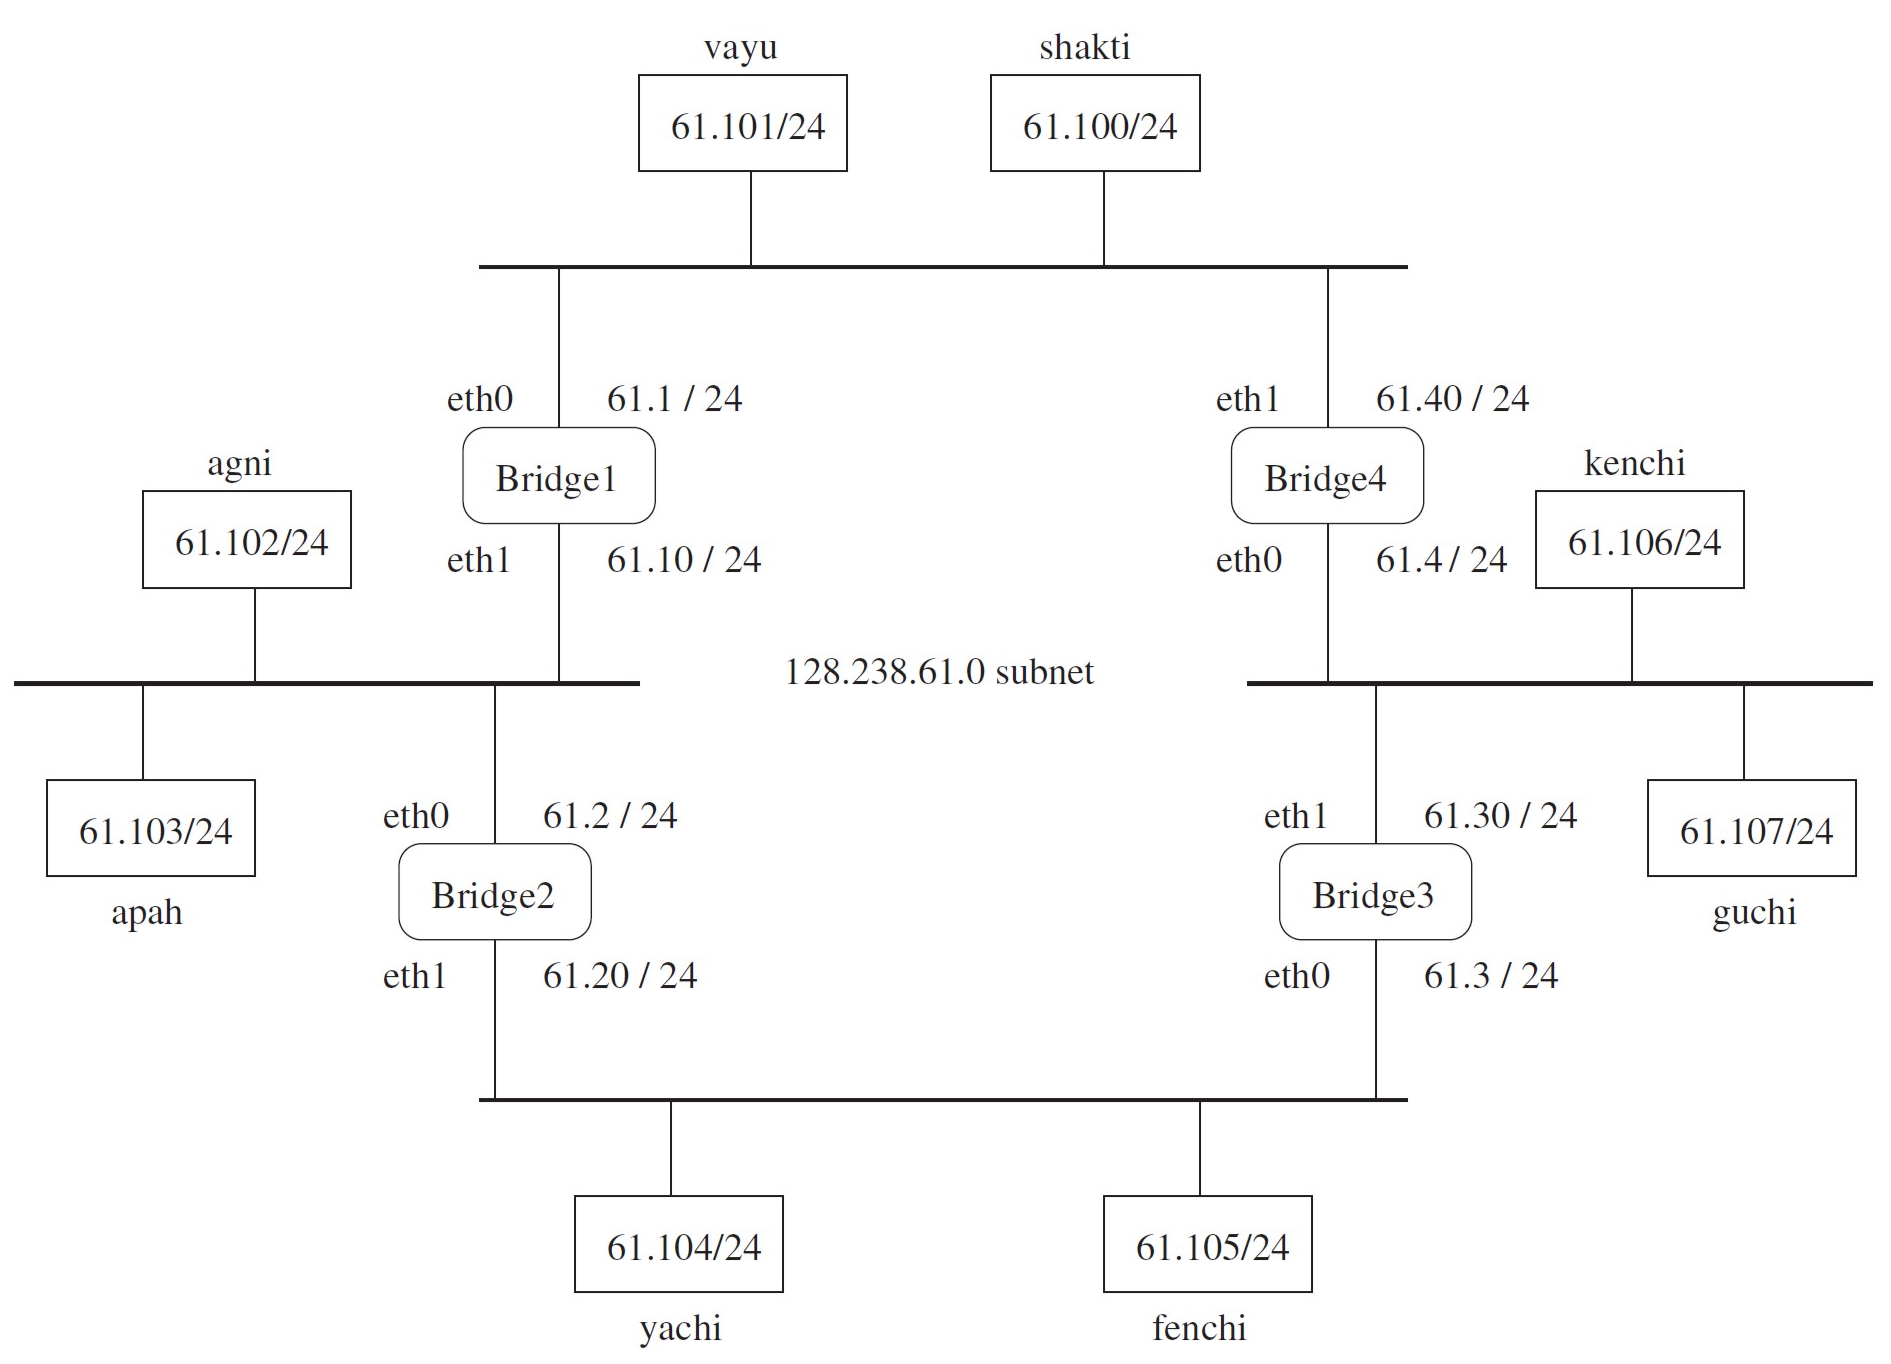
\includegraphics[width=0.9\textwidth]{img/figure3-8.png}
        \caption{\textit{Figure 3.8.} Bridge experiment network.}
    \end{figure}

\section{Multi bridge path}
    After configuring the network in Fig. 3.8, login to the bridge.

    Get to the \textit{Privileged EXEC} mode. Type \lstinline[language={cisco}]{show bridge} to see the entries in the bridge forwarding database.

    Whenever you \lstinline{ping} or \lstinline{telnet} from your workstation to a host that is not in the table, observe how the filtering database in the bridge is expanded.

    You may use the \lstinline[language={cisco}, emph={group}]{clear bridge group} command to remove any learned entries from the filtering database, if you see a full filtering database or if you want to repeat the above exercise.

    \subsection*{Report}
    From the output of \lstinline{show bridge}, identify which bridge ports are blocked, and which ports are in the forwarding state for each bridge.

\section{STP process}
    Using \lstinline{tcpdump -ex ether multicast}, capture the BPDU packet flowing on your network segment.

    \lstinline{telnet} to the hosts in the other three LAN segments and execute the above \lstinline{tcpdump} command in the \lstinline{telnet} window to collect BPDUs sent there.

    Login to each bridge to collect the \lstinline[language={cisco}]{show bridge} outputs.
    
    \subsection*{Report}
    Submit the four different BPDUs you saved.
    Identify the values of root ID, root path cost, bridge ID, and port ID for each BPDU.

    Based upon the initial BPDUs saved in \href{sec:spanning-tree}{Spanning tree exercise}, draw the spanning tree seen by the BPDUs. Identify the root ports and the root path cost (in hop counts) for each bridge.
    Identify the designated bridge and the designated port for each LAN segment.
    Identify the state of each bridge port (blocking or forwarding).

    Don’t just assume that \textit{Bridge1} has the highest priority for the root bridge.
    Draw the spanning tree based upon your data (eight initial BPDUs).

    Write the final BPDUs you collected using the three-tuple format: \textit{{root ID, root path cost, bridge ID}}.

    Once you have the spanning tree, justify it using the four final BPDUs collected in this exercise and/or the output of the \lstinline[language={cisco}]{show bridge} command.


\section{STP over topology dynamics}
    First, send \lstinline{ping} messages from \textit{h3} to \textit{h4}, while \lstinline{tcpdump} is running.
    Let the two programs run during this exercise.

    Then, disconnect the cable from the \textit{ethernet0} port of \textit{Bridge2} from the hub, and get system time (\lstinline{date}, \lstinline{date '+%D %T.%N'} or \lstinline{date +%s%N} to get nano seconds) on \textit{h3} or \textit{h4} to get the current time.

    Observe the \lstinline{ping} and \lstinline{tcpdump} windows. When the connection is reestablished, get the \lstinline{time} again. How long does it take the spanning tree algorithm to react to the change in the topology?

    Once you can successfully reach other hosts, get to the bridges to run \lstinline[language={cisco}]{show bridge} to collect the port states. Also collect BPDUs from all the LAN segments as you did in the previous exercise.

    After every student has collected the required data, connect the cable to the original position. Again, measure the time it takes for the bridges to adapt to the new change.
    
    \subsection*{Report}
    Draw the new tree formed after the cable was disconnected, based on the BPDUs you collected in this exercise. Specify the state of each bridge port.

    \section*{Exercise on the Cisco IOS web browser UI}
\section{Cisco IOS HTTP rest API}
    In this section we create simple network with a router and one gui host with \textit{Internet Browser} (you can use \texttt{utnetlab-ipgui}). Set IP same as previous section for your network.

    You can also configure a router using the web browser UI. To enable the web server, login to the router and config as below  in the \textit{Global Configuration} mode. 

    \begin{lstlisting}[language={cisco}]
R1(config)# aaa new-model
R1(config)# aaa authentication login default local
R1(config)# aaa authorization exec default local
R1(config)# username netlab privilege 15 password netlab
R1(config)# ip http server
R1(config)# ip http secure-server
R1(config)# ip http authentication local
    \end{lstlisting}
    
    Next, start a web browser (e.g.\ \textit{Mozilla} in Linux, or \textit{Hotjava} in Solaris) in your host, and enter the IP address of the router interface. When prompted, enter \texttt{netlab} for password, and leave the \texttt{User Name} field blank. Then you can browse the router configuration web pages and configure the router there.

\end{document}